\section{Alternative Modelle}

Dieses Kapitel bietet einen Einblick in weiterführende mathematische Aspekte, die im Rahmen 
dieser Arbeit nicht im Detail behandelt werden.
Ausgangspunkt sind stochastische Differentialgleichungen (SDEs), welche die Grundlage für die 
Modellierung und Simulation allgemeiner zeitstetiger 
stochastischer Prozesse bilden. Die Herleitung von Itô-SDEs über Itô-Integrale wird skizziert. 
Unter Verwendung des SDE-Kalkühls werden alternative Modelle zur geometrischen brownschen Bewegung vorgestellt. 
Beispielhaft wird das CEV-Modell (Constant Elastic Variance) untersucht, implementiert
und mit der GBM verglichen.

\begin{bem}[Motivation Stochastischer Differentialgleichungen]

Im Kapitel 4 wurde ein Aktienkurs durch die zeitdiskrete Übergangsgleichung
$$S_{n+1} = S_n \big(1 + \mu \Delta t + \sigma \sqrt{\Delta t}\,\varepsilon_{n+1}\big)$$
modelliert. Ziel des folgenden Abschnitts ist es, den Grenzübergang $\Delta t \to 0$ zu betrachten,
um eine kontinuierliche Beschreibung der Kursdynamik zu erhalten. Dabei soll die stochastische Differentialgleichung
$$dS_t = \mu S_t\,dt + \sigma S_t\,dW_t$$
hergeleitet werden, deren Lösung die geometrische brownsche Bewegung ist. 
Anschaulich muss man sich nur noch von $\sqrt{\Delta t} \varepsilon_{n+1} \to dW_t$ überzeugen, wobei $W_t$ eine brownsche Bewegung ist.
Seien $\Delta t = T/n$ und $(\varepsilon_k)_{k\ge 1}$ i.i.d. mit $E(\varepsilon_k)=0$, $V(\varepsilon_k)=1$.
Definiere den skalierten Zufallsspaziergang
$$
W^{(n)}(t) := \sqrt{\Delta t}\sum_{k=1}^{\lfloor t/\Delta t\rfloor}\varepsilon_k,\qquad t\in[0,T].
$$
Dann gilt für jedes feste $t$ nach dem Zentralen Grenzwertsatz
$$
W^{(n)}(t)\ \to\ \mathcal N(0,t).
$$
Und nach Kapitel 4 konvergiert $W^{(n)}$ sogar gegen eine brownsche Bewegung $W$.

Insbesondere sind die diskreten Inkremente unabhängig und es gilt für $k=\lfloor t/\Delta t\rfloor$
$$
W^{(n)}(t+\Delta t)-W^{(n)}(t)\;=\;\sqrt{\Delta t}\,\varepsilon_{k+1}\ \sim\ \mathcal N(0,\Delta t).
$$
Mit $W^{(n)}\to W$ folgt damit für jedes $t$ die Verteilungskonvergenz der Inkremente
$$
\sqrt{\Delta t}\,\varepsilon_{k+1}
\;=\;W^{(n)}(t+\Delta t)-W^{(n)}(t)\ \to \ W_{t+\Delta t}-W_t,
$$
Durch Missbrauch der Notation erhält man
$$
\sqrt{\Delta t}\,\varepsilon_{n+1}\ \to\ dW_t.
$$
Ebenso gilt
$$\Delta t \to dt, \qquad S_{t + \Delta t} - S_t \to dS_t.$$
Schließlich kann die Übergangsgleichung als stochastische Differentialgleichung interpretiert werden.
\qed

\end{bem}

Formal werden stochastische Differentialgleichungen über das It\^o-Integral eingeführt. Dies wird 
im nächsten Abschnitt skizziert, für eine genaue Darstellung sei auf die Literatur 
verwiesen, z. B. Behrends (2013) \cite{behrends} oder Karatzas und Shreve (1991) \cite{karatzas_brownian_1991}.
Die Argumentation orientiert sich am sechsten Kapitel des Lehrbuchs von Behrends.

\subsection{Stochastische Differentialgleichungen}

Ziel dieses Abschnitts ist es, die heuristische Schreibweise
$$
dS_t \;=\; a(S_t,t)\,dt \;+\; b(S_t,t)\,dW_t
$$
zu präzisieren.

\begin{lemma}[Differenzierbarkeit der brownschen Bewegung]
Die Pfade der brownschen Bewegung sind fast-sicher nicht differenzierbar. \textit{Beweis.}
Es wird gezeigt, das der Differenzenquotient fast-sicher divergiert. Ohne Einschränkung (Selbstähnlichkeit) wird $t=0$ betrachtet. Für $n \in \Bbb N$ sei
$$\Delta_n W := \frac{W_{1/n} - W_0}{1/n}=n W_{1 / n} \sim \mathcal N(0, n).$$
Für jedes $M \gt 0$ gilt daher (analoge Abschätzung in Kap. 3)
$$P(\vert \Delta_n W \vert \lt M) \lt 2 \exp(- \frac{M^2}{2 n}).$$
Für $n \to \infty$ konvergiert somit die Summe der Wahrscheinlichkeiten mit $M_n = 2^n$, und wegen dem Lemma von Borel-Cantelli
folgt die Behauptung. \qed
\end{lemma}

Wie kann man nun eine Differenzialgleichung definieren, wenn die vorliegenden Objekte nicht differenzierbar sind? Genauso wie man eine klassische Differentialgleichung, z. B
$$dy = f(y)$$
durch die Integralgleichung
$$y = \int f(y)$$
beschreiben kann, so auch It\^o-SDEs mit stochastischen Integralen (It\^o-Integralen).
Arbeitsraum ist ein filtrierter Wahrscheinlichkeitsraum
$$
(\Omega,\mathcal F,(\mathcal F_t)_{t\ge 0},P),
$$
und es sei $W_t$ eine brownsche Bewegung. 

Analog zu analytischen Integralen wird das stochastische Integral über Treppenfunktionen definiert:
Genauso wie eine integrierbare Funktion 
durch eine Folge von Stufen approximiert wird, werden stochastische Prozesse durch elementare Prozesse angenähert.

\begin{bem}[Vorhersagbare Prozesse]
Die Klasse der \textit{vorhersagbaren} stochastischen Prozesse bildet eine Erweiterung der links-stetigen Prozesse, so dass 
z. B. auch Poisson-Prozesse (sprunghaft) zugelassen werden (\cite{karatzas_brownian_1991} S. 131).
Stochastische Integrale und somit auch SDEs werden für solche Prozesse definiert. U. A. gilt: Vorhersagbar impliziert Adaptiert.
Naturanaloge Prozesse sind meist vorhersagbar: Wenn man das Wetter jetzt kennt, so auch (ungefähr) in einer Minute.
\end{bem}

\begin{defi}[Elementare Prozesse und ihr Integral]
Fixiere $T>0$. Ein Prozess $H$ heißt \emph{elementar} auf $[0,T]$, wenn es eine 
Zerlegung $0=t_0<t_1<\dots<t_n=T$ und Zufallsvariablen $\xi_i\in L^2(\Omega,\mathcal F_{t_i},\mathbb P)$, $i=0,\dots,n-1$, gibt mit
$$
H_t \;=\; \sum_{i=0}^{n-1} \xi_i\,\mathbf 1_{(t_i,t_{i+1}]}(t),\qquad t\in[0,T].
$$
Für solche $H$ definiert das \emph{It\^o-Integral} gegen $W$ durch
$$
\int_0^T H_s\,dW_s \;:=\; \sum_{i=0}^{n-1} \xi_i\,\big(W_{t_{i+1}}-W_{t_i}\big).
$$
Zentrale Eigenschaften sind
\begin{equation}\label{eq:ito_isometry}
E\!\left[\int_0^T H_s\,dW_s\right] \;=\; 0,\qquad
E\!\left[\Big(\int_0^T H_s\,dW_s\Big)^{\!2}\right] \;=\; E\!\left[\int_0^T H_s^2\,ds\right].
\end{equation}
Dies ist die \emph{It\^o-Isometrie}. Mit der It\^o-Isometrie kann man aus quadratintegrablen Prozessen
schließen, dass das It\^o-Integral existiert. Der entstandene Prozess in $T$ ist ein Martingal.
\end{defi}

\begin{satz}[Dichtheit der elementaren Prozesse]
Die Frage, wann ein stochastischer Prozess durch einen elementaren Prozess approximierbar ist wird im Folgenden 
beantwortet. Das wird wie folgt ausgedrückt: Die Menge der elementaren Prozesse liegt \textit{dicht} im Raum
der quadratintegrierbaren Prozesse. Dann gibt es zu jedem stochastischen Prozess einen elementaren stochastischen
Prozess, deren Integrale sich um ein beliebiges $\varepsilon$ unterscheiden.

Sei $L^2_{\mathrm{pred}}(\Omega\times[0,T])$ der Funktionen-Raum aller vorhersagbaren Prozesse $X$ mit der Norm
\begin{equation}\label{eq:ito_norm}
\|X\|_{2,T}^2 := E \left [ \int_0^T |X_s|^2 ds \right ] < \infty.  
\end{equation}

Dann ist die Klasse der elementaren vorhersagbaren Prozesse dicht 
in $L^2_{\mathrm{pred}}(\Omega\times[0,T])$ bezüglich der Norm $\|\cdot\|_{2,T}$. (Siehe z. B. Karatzas und Shreve \cite{karatzas_brownian_1991}, S. 132f.) 
Die Dichtheit garantiert, dass zu einem beliebigen (vorhersagbaren, quadratintegrierbaren) Prozess 
eine Folge von elementaren Prozessen existiert, die dagegen konvergiert.
\end{satz}

\begin{defi}[It\^o-Integral]
Das It\^o-Integral ist nun für elementare Prozesse definiert, und für einen beliebigen Prozess existiert
eine passende Folge. So wird dann das It\^o-Integral für beliebige Prozesse definiert:
Das It\^o-Integral ist der Grenzwert der Integrale der approximierenden elementaren Prozesse.
Offen bleibt aber die Frage nach der Wohldefiniertheit dieses Integral-Begriffs. Konvergieren zwei Folgen $G_t^{(n)}$, $H_t^{(n)}$ von
elementaren Prozessen gegen einen Prozess $X_t$ (in der Norm $\|\cdot\|_{2,T}^2$), so muss auch das Integral im Grenzwert übereinstimmen.
Hier wird die oben genannte It\^o-Isometrie genutzt.

Für einen allgemeinen vorhersagbaren Prozess $X\in L^2_{\mathrm{pred}}(\Omega\times[0,T])$ wähle 
eine Folge elementarer Prozesse $H^{(n)}$ mit
$\|H^{(n)}-X\|_{2,T}\to 0$. Dann definiert man
$$
\int_0^T X_s\,dW_s \;:=\; L^2\text{-}\lim_{n\to\infty}\;\int_0^T H^{(n)}_s\,dW_s,
$$
wobei der Limes aufgrund der It\^o-Isometrie existiert und nicht von der approximierenden Folge abhängt:
Für zwei Folgen $G$ und $H$ gilt
$$
\begin{aligned}
E\!\left[
   \left( \int_0^T \big(H^{(n)}_s - G^{(n)}_s\big)\,dW_s \right)^2
\right]
&\overset{\ref{eq:ito_isometry}}{=}
E \left [ \int_0^T \big(H^{(n)}_s - G^{(n)}_s\big)^2\,ds \right ].
\\ &\overset{\ref{eq:ito_norm}}{=} \|H^{(n)} - G^{(n)}\|_{2,T}^2
\end{aligned}
$$
Wegen der Dreiecksungleichung folgt
$$
\|H^{(n)} - G^{(n)}\|_{2,T} 
\;\le\; 
\|H^{(n)} - X\|_{2,T} + \|G^{(n)} - X\|_{2,T}
\;\to\; 0.
$$
Somit gilt
$$
\int_0^T H^{(n)}_s\,dW_s - \int_0^T G^{(n)}_s\,dW_s 
\;\to\; 0 \quad \text{in } L^2(\Omega).
$$
Daher ist das It\^o-Integral wohldefiniert. \qed \\
Für jedes $t\in[0,T]$ definiert man analog den Prozess
$$
\Big(\int_0^t X_s\,dW_s\Big)_{t\in[0,T]},
$$
und es gilt weiterhin die It\^o-Isometrie
$$
E\!\left[\Big(\int_0^T X_s\,dW_s\Big)^{\!2}\right] \;=\; E\!\left[\int_0^T X_s^{2}\,ds\right],
$$
sowie die Martingaleigenschaft von $M_t:=\int_0^t X_s\,dW_s$. Für lokal 
quadratintegrierbare $X$ erhält man das Integral durch Lokalisierung via Stoppzeiten.
\end{defi}

\begin{defi}[Stochastische Differentialgleichungen]
Mit dieser Konstruktion ist die Schreibweise
$$
dS_t \;=\; a(S_t,t)\,dt \;+\; b(S_t,t)\,dW_t
$$
präzise zu lesen als Integralgleichung
$$
S_t \;=\; S_0 \;+\; \int_0^t a(S_s,s)\,ds \;+\; \int_0^t b(S_s,s)\,dW_s,
$$
wobei $b(S_\cdot,\cdot)$ vorhersagbar und quadratintegrierbar sein muss. Diese Klasse der SDEs werden auch It\^o-SDEs genannt.
$a$ nennt man Drift-Term und $b$ nennt man Diffusionsterm.
\end{defi}

\subsection{Charakterisierung alternativer Kursmodelle durch stochastische Differentialgleichungen}

Die GBM nimmt konstante Volatilität und lognormale Renditen an; sie erzeugt weder 
Sprünge noch Volatilitäts-Clustering oder kann Konjunkturperioden Modellieren.
Glasserman \cite{glasserman2003monte} beschreibt verschiedene Ansätze zur Modellierung solcher Phänomene. 

\begin{bsp}[Lokale Volatilität]
Deterministisch zeit- und zustandsabhängige Volatilität:
$$
dS_t \;=\; \mu(t,S_t)\,S_t\,dt \;+\; \sigma_{\mathrm{loc}}(t,S_t)\,S_t\,dW_t.
$$
Spezialfall CEV:
$$
dS_t \;=\; \mu S_t\,dt \;+\; \sigma\,S_t^{\beta}\,dW_t,\qquad \beta\in\mathbb R,
$$
wodurch die Volatilität bei kleinen/größeren Preisen relativ ansteigt/abnimmt.
\end{bsp}

\begin{bsp}[Stochastische Volatilität]
Volatilität ist selbst ein Zufallsprozess.
$$
\begin{aligned}
dS_t &= \mu S_t\,dt + \sqrt{V_t}\,S_t\,dW_t^{(1)},\\
dV_t &= \kappa(\theta - V_t)\,dt + \xi\sqrt{V_t}\,dW_t^{(2)},\quad d \langle W^{(1)},W^{(2)}\rangle_t=\rho\,dt,
\end{aligned}
$$
mit Feller-Bedingung $2\kappa\theta\ge \xi^2$ für Positivität von $V_t$.
\end{bsp}

\begin{bsp}[Sprung-Diffusions-Modelle]
Diffusion mit seltenen Sprüngen modelliert durch Poisson-Prozesse.
$$
\frac{dS_t}{S_t} \;=\; \big(\mu - \lambda \kappa_J\big)\,dt \;+\; \sigma\,dW_t \;+\; (J_t-1)\,dN_t,
$$
wobei $N_t$ Poisson mit Intensität $\lambda$ ist, $J_t$ die Sprunggröße (z.\,B. lognormal) 
und $\kappa_J= E(J_t-1)$; der Driftterm kompensiert die Sprünge.
\end{bsp}

\subsection{Simulation stochastischer Prozesse}
Zu einer SDE
$$
dX_t \;=\; a(X_t,t)\,dt \;+\; b(X_t,t)\,dW_t,\quad t\in[0,T],
$$
wird ein Zeitschrittgitter $t_n=n\Delta t$ eingeführt und der kontinuierliche Prozess durch eine zeitdiskrete Approximation ersetzt. Erwartungswerte werden via Monte‑Carlo über viele simulierte Pfade geschätzt.

Die Differentialgleichung (DGL) wird mit Euler (deterministisch) und Euler–Maruyama (stochastisch) diskretisiert (vgl. Bärwolff \cite{Baerwolff2025} u. a. S. 269, 466f.).
Für die DGL $x^\prime(t)=a(x(t),t)$ liefert das explizite Euler‑Schema
$$
x_{n+1} \;=\; x_n \;+\; a(x_n,t_n)\,\Delta t.
$$
Ersetzt man nun formal $dW_t$ durch $\Delta W_n:=W_{t_{n+1}}-W_{t_n}\sim \mathcal N(0,\Delta t)$, erhält man die natürliche stochastische Erweiterung, das Euler–Maruyama‑Schema:
$$
\begin{aligned}
X_{n+1} \;&=\; X_n \;+\; a(X_n,t_n)\,\Delta t \;+\; b(X_n,t_n)\,\Delta W_n \\
\;&=\; X_n \;+\; a(X_n,t_n)\,\Delta t \;+\; b(X_n,t_n)\,\sqrt{\Delta t}\,\varepsilon_{n+1},
\end{aligned}
$$
mit i.i.d. $\varepsilon_{n}\sim\mathcal N(0,1)$. 
Ähnlich wurde im Hauptteil die geometrische brownsche Bewegung hergeleitet.

\begin{bsp}[Implementierung]
Es folgt ein R-Programm zur Simulation eines CEV-Modells (s. u.).

\begin{lstlisting}
simulate_cev_paths <- function(S0, mu, sigma, beta, dt, nsteps, npaths) {
  S <- matrix(NA, nrow = nsteps + 1, ncol = npaths)
  S[1, ] <- S0
  for (i in 1:nsteps) {
    Z <- rnorm(npaths)
    S[i+1, ] <- S[i, ] + mu * S[i, ] * dt + sigma * (S[i, ]^beta) * sqrt(dt) * Z
    S[i+1, ][S[i+1, ] <= 0] <- 1e-8
  }
  return(S)
}
\end{lstlisting}

\end{bsp}

\subsection{Implementierung eines CEV (Constant Elasticity of Variance) Modell}
Das CEV-Modell ist ein Spezialfall der lokalen Volatilität mit
$$
dS_t \;=\; \mu\,S_t\,dt \;+\; \sigma\,S_t^{\beta}\,dW_t,\qquad \beta\in\mathbb R.
$$
\begin{itemize}
\item $\beta=1$ ergibt GBM. 
\item $\beta<1$ erhöht die relative Volatilität bei kleinen Preisen.
\item $\beta>1$ verstärkt Schwankungen bei hohen Preisen.
\end{itemize}
Mit diskreten Beobachtungen $S_{t_i}$ im Abstand $\Delta t$ liefert das Euler‑Schema
$$
\Delta S_i \approx \mu S_{t_i}\Delta t + \sigma S_{t_i}^{\beta}\sqrt{\Delta t}\,\varepsilon_i,\quad \varepsilon_i\sim\mathcal N(0,1).
$$
Die nächste Herausforderung ist die Kalibrierung (Parameterschätzung) aus gegebenen Daten. Die Arbeit 
orientiert sich im folgenden an Iacus (2008, S. 122 ff.) \cite{iacus2008}. Eine eigene Implementierung in
R wird danach mit dem Softwarepaket Sim.DiffProc \cite{rsde} (2020) verglichen, das man auf den selben Ansatz konfigurieren kann.
Der Ansatz ist die numerische Maximierung einer Log-Likelihood-Funktion, die im Folgenden 
für die diskrete Übergangswahrscheinlichkeit hergeleitet wird.
Das wird durch die Approximation der Übergangsdichte (eine bedingte Dichte) mittels des 
Euler-Maruyama-Schemas erreicht. Da sich für $\beta=1$ eine klassische geometrische brownsche Bewegung ergibt, 
können die bekannten Schätzer für Drift und Volatilität als Spezialfall betrachtet werden. Insbesondere stellen die Parameter der GBM 
sinnvolle Startwerte für die numerische Optimierung dar.

\begin{lemma}[(Quasi) Maximum-Likelihood-Schätzung (MLE, QMLE)]
Ziel ist die Parameterschätzung aus diskreten Beobachtungen $S_{t_0},\dots,S_{t_n}$ eines SDE
$dS_t=a(S_t,t)\,dt+b(S_t,t)\,dW_t$. Grundidee: Wähle Parameter $\theta$ so, dass die beobachteten 
Daten unter dem Modell am wahrscheinlichsten sind. Für diskrete Beobachtungen $S_{t_0},\dots,S_{t_n}$ eines (Markov‑)Modells gilt
$$
L(\theta) \;=\; \prod_{i=0}^{n-1} p_\theta\!\big(S_{t_{i+1}},\,\Delta t \,\big|\, S_{t_i}\big), 
\qquad
\ell(\theta)=\log L(\theta)=\sum_{i=0}^{n-1}\log p_\theta\!\big(S_{t_{i+1}},\Delta t \,\big|\, S_{t_i}\big),
$$
wobei $p_\theta(\,\cdot\,|\,\cdot)$ die bedingte Übergangsdichte in Schrittweite $\Delta t$ ist. Der MLE ist
$$
\widehat\theta\;=\;\underset{\theta}{\arg\max}\ \ell(\theta).
$$
Da $p_\theta$ (hier) nicht explizit bekannt ist, wird eine Quasi-Likelihood (QMLE)-Methode verwendet. 
Hier mit Hilfe der Euler-Maruyama-Approximation.
$$
S_{t_{i+1}}-S_{t_i}\mid S_{t_i}\ \approx\ \mathcal N\!\big(a_\theta(S_{t_i},t_i)\,\Delta t,\; b_\theta^2(S_{t_i},t_i)\,\Delta t\big),
$$
Anschließend wird die (Pseudo‑)Log‑Likelihood aufgestellt und numerisch maximiert.
\end{lemma}

\begin{satz}[Quasi‑MLE für das CEV Modell (Euler‑Pseudo‑Likelihood)]
Das CEV-Modell lautet
$$
dS_t = \mu S_t\,dt + \sigma S_t^{\beta}\,dW_t.
$$
Für kleine Zeitschritte $\Delta t$ wird die Differentialgleichung diskretisiert:
$$
S_{t_{i+1}} \approx S_{t_i} + \mu S_{t_i} \Delta t + \sigma S_{t_i}^{\beta} \sqrt{\Delta t}\, \varepsilon_{i+1},
$$
wobei $\varepsilon_{i+1} \sim \mathcal N(0,1)$ unabhängig sind.
Definiere die Inkremente:
$$
\Delta S_i := S_{t_{i+1}} - S_{t_i}
$$
Nach obiger Diskretisierung gilt näherungsweise (in die man die deterministischen Terme in die Verteilung von $\varepsilon$ reinzieht):
$$
\Delta S_i \mid S_{t_i} \sim \mathcal N\left(\mu S_{t_i} \Delta t,\, \sigma^2 S_{t_i}^{2\beta} \Delta t\right)
$$
Das heißt: Für gegebenen Kurs $S_{t_i}$ ist der nächste Schritt normalverteilt mit 
Mittelwert $\mu S_{t_i} \Delta t$ und Varianz $\sigma^2 S_{t_i}^{2\beta} \Delta t$.
Die Dichte einer Normalverteilung mit Mittelwert $m$ und Varianz $v$ an der Stelle $x$ ist:
$$
p(x) = \frac{1}{\sqrt{2\pi v}} \exp\left(-\frac{(x-m)^2}{2v}\right)
$$
Setze $m = \mu S_{t_i} \Delta t$, $v = \sigma^2 S_{t_i}^{2\beta} \Delta t$, $x = \Delta S_i$.
Die gemeinsame Likelihood für alle Schritte ist das Produkt der Einzeldichten:
$$
L(\mu, \sigma, \beta) = \prod_{i=0}^{n-1} p(\Delta S_i \mid S_{t_i})
$$
Da Produkte numerisch unhandlich sind, nimmt man den Logarithmus:
$$
\ell(\mu, \sigma, \beta) = \sum_{i=0}^{n-1} \log p(\Delta S_i \mid S_{t_i})
$$
Setzt man die Dichte $p$ ein, ergibt sich die Likelihood
\begin{align*}
\ell(\mu, \sigma, \beta) &= \sum_{i=0}^{n-1} \left[
    -\frac{1}{2} \log(2\pi \sigma^2 S_{t_i}^{2\beta} \Delta t)
    -\frac{(\Delta S_i - \mu S_{t_i} \Delta t)^2}{2 \sigma^2 S_{t_i}^{2\beta} \Delta t}
\right] \\
&= -\frac{1}{2} \sum_{i=0}^{n-1} \left[
    \log(2\pi \sigma^2 S_{t_i}^{2\beta} \Delta t)
    + \frac{(\Delta S_i - \mu S_{t_i} \Delta t)^2}{\sigma^2 S_{t_i}^{2\beta} \Delta t}
\right]
\end{align*} 
\qed
\end{satz}

\begin{bem}[Interpretation]
Die Log-Likelihood misst, wie gut die Parameter $(\mu, \sigma, \beta)$ die beobachteten Kursänderungen erklären. 
Der erste Term bestraft große Varianzen, der zweite Term misst die Abweichung der beobachteten Inkremente von den erwarteten Werten.
Die Schätzungen der Parameter erhält man durch Maximierung der Log-Likelihood:
$$
(\widehat{\mu}, \widehat{\sigma}, \widehat{\beta}) = \underset{\mu, \sigma, \beta}{\arg\max} \; \ell(\mu, \sigma, \beta)
$$
Die Funktion wird mit numerischen Optimierungsverfahren (z.B. L-BFGS-B) maximiert.
\end{bem}

\begin{bsp}[Implementierung in R mit dem Paket Sim Diffproc]
Die Parameterschätzung für das CEV-Modell kann mit dem R-Paket Sim.DiffProc durchgeführt werden. Die 
Funktion \texttt{fitsde} erlaubt die Schätzung der Drift- und Diffusionsparameter mittels 
Pseudo-Maximum-Likelihood auf Basis diskreter Zeitreihen. Das folgende R-Programm (Ausschnitt) zeigt die Anwendung auf DAX-Daten.
Die Optimierung erfolgt mit dem Algorithmus L-BFGS-B und die Parametergrenzen sind gesetzt, um numerische Probleme zu vermeiden.

\begin{lstlisting}
S_ts <- ts(dax$Price, deltat = dt_daily)

drift     <- expression(theta[1] * x)           # theta1 = mu
diffusion <- expression(theta[2] * x^theta[3])    # theta2 = sigma, theta3 = beta

fit_cev <- fitsde(
  data      = S_ts,
  drift     = drift,
  diffusion = diffusion,
  start     = start_vals,
  pmle      = "euler",
  optim.method = "L-BFGS-B",
  lower     = c(mu = -Inf, sigma = 1e-8, beta = 0.0),
  upper     = c(mu =  Inf, sigma =  Inf, beta = 3.0)
)
\end{lstlisting}

Es folgt ein Backtest mit den geschätzten Parametern (vgl. Kapitel 7). Hier werden 1000 Pfade mit der
Euler-Maruyama-Methode simuliert und anschließend die empirischen 50\%-Quantile genommen.

\begin{figure}[H]
    \centering
    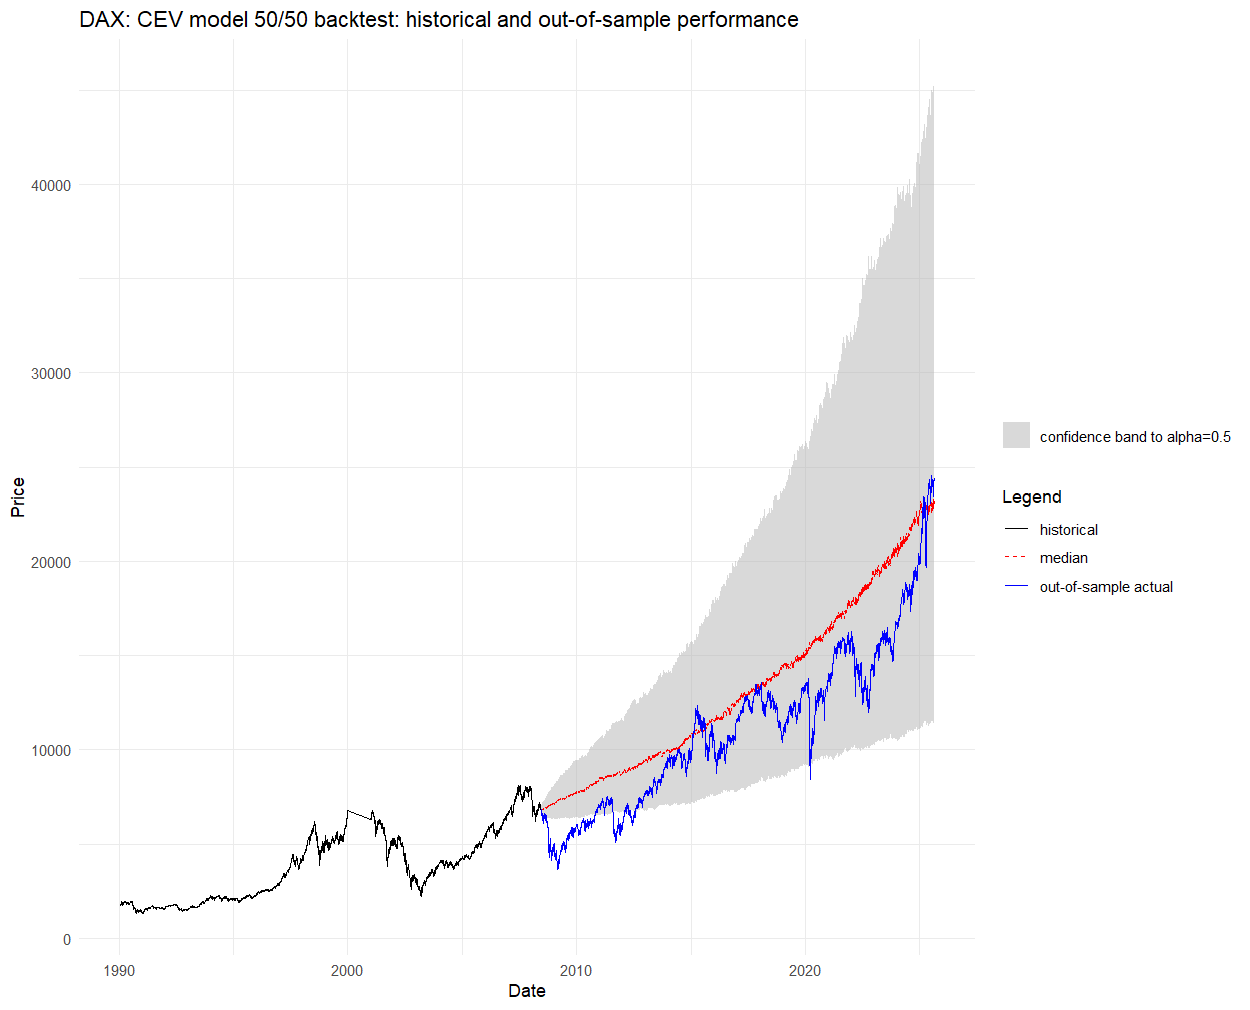
\includegraphics[width=0.9\textwidth]{images/cev_dax_backtest.png}
    \caption{Backtest CEV-Modell für den DAX}
    \label{fig:cev_dax_backtest}
\end{figure}

Die Überdeckungswahrscheinlichkeit liegt bei 82\%. Dieselbe Konfiguration
lieferte für die gemetrische brownsche Bewegung eine Überdeckungswahrscheinlichkeit von 86\% (größer ist besser).
Ein feinerer Vergleich der Kalibrierungen folgt im nächsten Abschnitt. 

\end{bsp}

\begin{bsp}[Eigene Implementierung in R mit der Euler‑Pseudo‑Likelihood]
Die eigene Implementierung der Parameterschätzung für das CEV-Modell in R basiert auf der oben hergeleiteten 
Pseudo-Maximum-Likelihood-Funktion.
Zur numerischen Optimierung wird das Paket nloptr \cite{nlopt} verwendet.

\begin{lstlisting}
estimate_cev <- function(S, dt = 1/252) {
  S <- as.numeric(S)
  stopifnot(is.numeric(S), all(is.finite(S)), length(S) >= 3)
  
  dS  <- diff(S)
  S0  <- S[-length(S)]
  eps <- 1e-12
  S0[S0 <= 0] <- eps
  sigma_start <- sd(dax_in$logret)  / sqrt(dt_daily)
  mu_start    <- mean(dax_in$logret) / dt_daily - sigma_start / 2
  beta_start  <- 1.0
  init <- c(mu_start, sigma_start, beta_start) 
  
  negloglik <- function(par) {
    mu    <- par[1]
    sigma <- par[2]
    beta  <- par[3]
    if (!is.finite(mu) || !is.finite(sigma) || !is.finite(beta)) return(1e12)
    if (sigma <= 0 || beta <= 0 || beta >= 5) return(1e12)
    
    denom <- (sigma*sigma) * (S0^(2*beta)) * dt
    denom[denom <= 0] <- eps
    val <- 0.5 * sum(log(2*pi*denom) + ((dS - mu*S0*dt)^2)/denom)
    if (!is.finite(val)) val <- 1e12
    as.numeric(val)
  }
  
  res <- nloptr(
    x0     = init,
    eval_f = negloglik,
    lb     = c(-Inf, 1e-8, 1e-6),
    ub     = c( Inf,  Inf,  4.999),
    opts   = list(algorithm = "NLOPT_LN_SBPLX", xtol_rel = 1e-8, maxeval = 3000)
  )
  
  list(mu = res$solution[1], sigma = res$solution[2], beta = res$solution[3])
}
\end{lstlisting}


\paragraph{Vergleich der Kalibrierungen}
Im Vergleich des Standardpakets mit der eigenen Implementierung zeigt sich, dass die geschätzten Parameter
bloß geringe Unterschiede aufweisen. Man kann schließen, dass die Schätzung korrekt implementiert ist.

\begin{table}[H]
\centering
\caption{Vergleich der geschätzten Parameter ($\mu$, $\sigma$, $\beta$) für die beiden Schätzprogramme}
\label{tab:compare_models_ab}
\begin{tabular}{lcccccc}
\hline
 & \multicolumn{3}{c}{Eigene Implementierung} & \multicolumn{3}{c}{Paket} \\
\cline{2-4}\cline{5-7}
Kurs & $\mu$ & $\sigma$ & $\beta$ & $\mu$ & $\sigma$ & $\beta$ \\
\hline
DAX & $0.0946$ & $0.6545$ & $0.8726$ & $0.0950$ & $0.6524$ & $0.873$ \\
Lufthansa & $0.003$ & $0.8483$ & $0.6423$ & $0.0035$ & $0.8484$ & $0.6423$ \\
Adesso & $0.2686$ & $0.4114$ & $1.0031$ & $0.2686$ & $0.4122$ & $1.0026$ \\
\hline
\end{tabular}
\end{table}
\end{bsp}

\subsection{Ergebnisse und Vergleich der Modelle}

Nun wird das CEV-Modell (unter Verwendung der in Sim.Diffproc vorgenommenen Kalibrierung) mit der geometrischen brownschen Bewegung (GBM) verglichen. (Siehe Anhang B.) Beide Modelle werden auf denselben Datensatz angewendet und anschließend in einem Backtest bewertet.

Zum Einen erfolgt eine Aufteilung der Daten nach einem bestimmten Gewicht (weight): Das Modell wird auf Basis der 
historischen Daten kalibriert und anschließend zur Prognose der zukünftigen Daten eingesetzt. Die Prognosegüte 
wird gemessen und über alle Gewichte hinweg als Mittelwert angegeben.
Zum Anderen wird ein sequentieller Backtest mit einem festen Zeitintervall von 20 Tagen durchgeführt, bei dem jeweils 
alle bis dahin verfügbaren Daten zur Prognose herangezogen werden.


\paragraph{Interpretation der Ergebnisse}
Für den DAX zeigen GBM und CEV ein sehr ähnliches Verhalten. Die Prognosequalität verbessert sich erwartungsgemäß 
mit zunehmendem Gewicht. Dies steht im Einklang mit der Parameterschätzung, da $\beta$ nahe bei $1$ liegt (s. o.) und 
sich das CEV-Modell in diesem Fall nahezu wie eine GBM verhält.
Auch bei der Lufthansa-Aktie liefern beide Modelle vergleichbare, jedoch insgesamt schlechtere Ergebnisse, da der 
Kurs (anders als beim DAX) keinen (log-)linearen Trend aufweist.
Als Beispiel für eine ausgeprägte Korrelation zwischen Preis und Volatilität, bei der das CEV-Modell 
Vorteile bietet, wird der Wechselkurs der türkischen Lira gegenüber dem US-Dollar während der Finanzkrise 2021 untersucht (vgl. Abbildung \ref{fig:cev_try}). Hier zeigt das CEV-Modell eine deutliche Verbesserung.

\begin{figure}[H]
    \centering
    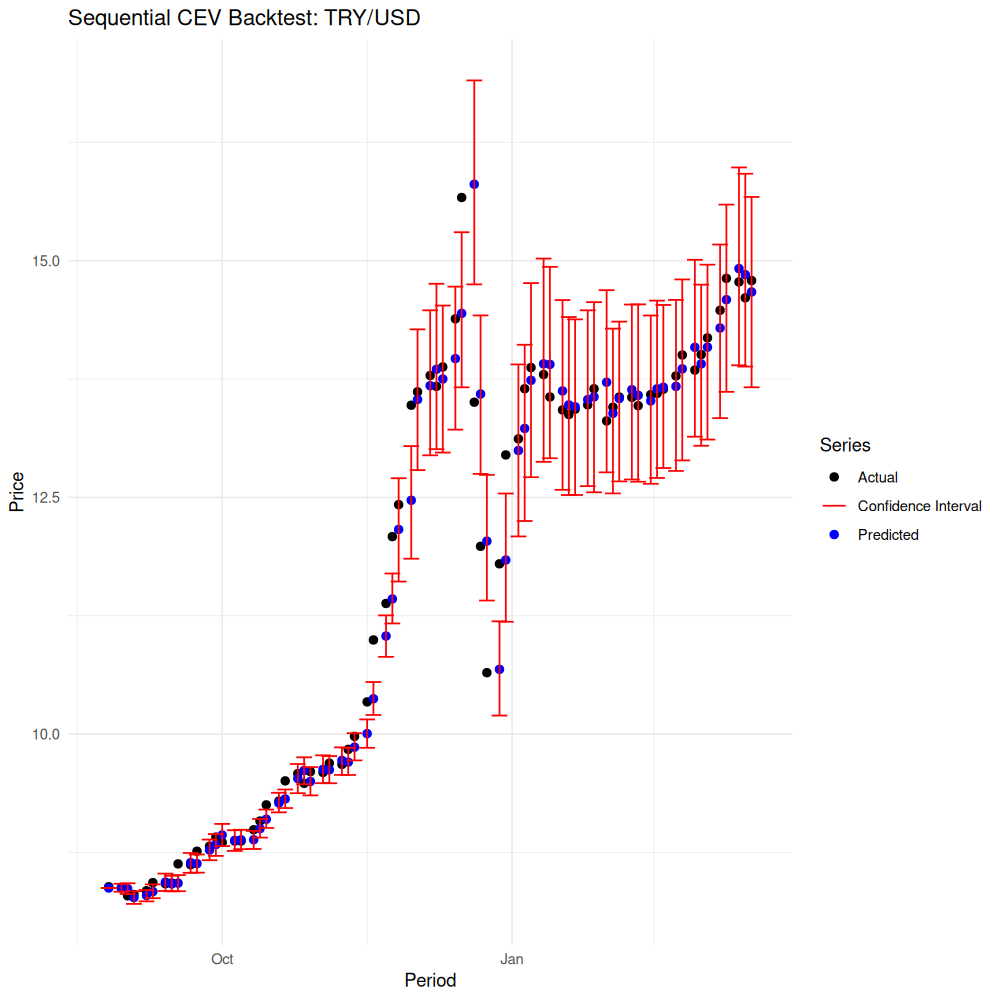
\includegraphics[width=0.9\textwidth]{images/cev_try.png}
    \caption{Sequenzieller Backtest des CEV Modell für die türkische Lira (Wechselrate Dollar), Abstand von 2 Tagen während der türkischen Finanzkrise 2021}
    \label{fig:cev_try}
\end{figure}